\documentclass[11pt,twoside]{article}
\usepackage{fullpage,lscape,graphicx,setspace,multicol,sidecap}
\renewcommand{\thesection}{\arabic{section}}
\begin{document}

\begin{titlepage}

 \begin{center}

 \uppercase{  {\Large Multi-method  detrital  thermochronology of  the
               Great Valley Group near New Idria, California}  }

Pieter Vermeesch\footnote
{\small Department of Geological and Environmental Sciences, Stanford University\\
Braun Hall, room 320-305, 450 Serra Mall,\\
Stanford, CA 94305-2115\\ 
pvermees@pangea.stanford.edu}, 
Donald D. Miller \footnote
{\small Aera Energy, LLC, P.O. Box 11164\\ 
Bakersfield, CA 93389-1164\\
ddmiller@aeraenergy.com}, 
Stephan A. Graham\footnote
{\small Department of Geological and Environmental Sciences, Stanford University\\
Braun Hall, room 320, 450 Serra Mall,\\
Stanford, CA 94305-2115\\ 
graham@pangea.stanford.edu},
Johan De Grave\footnote
{\small Geological Institute, University of Gent,\\ 
Krijgslaan 281, B-9000 Gent, Belgium\\
johan.degrave@ugent.be},
Michael O. McWilliams\footnote
{\small Department of Geological and Environmental Sciences, Stanford University\\
Braun Hall, room 320, 450 Serra Mall,\\
Stanford, CA 94305-2115\\ 
mcwilliams@stanford.edu}\\

Keywords: detrital thermochronology, fission tracks, Great Valley Group, serpentinite, 
Sierra Nevada, exhumation

 \end{center}

 \end{titlepage}

\begin{abstract}
The  simultaneous  use   of  several  thermochronological  methods  on
replicate  sedimentary   rock  samples  can  reveal   their  pre-  and
post-depositional history.  Single grain U/Pb dating of zircon, zircon
and   apatite   fission  track   dating   and  vitrinite   reflectance
measurements were performed  on Cretaceous through Miocene sedimentary
rocks  of  the Great  Valley  Group  and  the Temblor  Formation  near
Coalinga and  New Idria,  California.  The data  show that  the Sierra
Nevada was exhumed and  cooled at $\sim$0.5-1km/Ma or $\sim$20$^o$C/Ma
during the  Cretaceous.  After deposition in the  Great Valley forearc
basin,  Sierra Nevada erosional  products were  buried at  great depth
under low thermal gradients.  At $\sim$12-14 Ma, northward progression
of  the Mendocino  triple junction  triggered folding  on  the eastern
flanks of the California Coast  Ranges and rapid exhumation of the New
Idria  serpentinite  diapir.  This  Middle   Miocene  event caused  the
deposition  of spectacular deposits  of sedimentary  serpentinite (Big
Blue Formation).  The rapid rise  of the hot serpentinite body created
a thermal pulse  that may have provided the  enigmatic heat source for
oil fields in the shallow  Vallecitos syncline, a few kilometers north
of New Idria.
\end{abstract}

\section*{\uppercase{Introduction}}
\label{sec:introduction}

The  topography and  geology of  central California  are  dominated by
petrotectonic elements  of the Mesozoic convergent  margin: the Sierra
Nevada  magmatic  arc,  the   Great  Valley  forearc  basin,  and  the
Franciscan  accretionary prism.  These  three domains  are genetically
linked,  inasmuch  as  they  were  jointly  formed  by  Pacific  plate
subduction  beginning in the  Late Jurassic  (Dickinson {\it  et al.},
1996),  until  the  transformation  of  the  subduction  zone  into  a
transform margin during the  Late Cenozoic (Atwater, 1970).  The upper
Mesozoic strata of the Great Valley Group (or Sequence: Bailey {\it et
al.}, 1964) filled the forearc basin, and comprise one of the thickest
sequences  of  Cretaceous sediments  known  (Ingersoll, 1982).   These
Great Valley  Group strata crop out  in a homocline  along the western
margin of California's  Central Valley, and are in  fault contact with
the Franciscan accretionary complex (Dickinson {\it et al.}, 1996).\\

  \begin{figure}[here]
  \begin{center}
  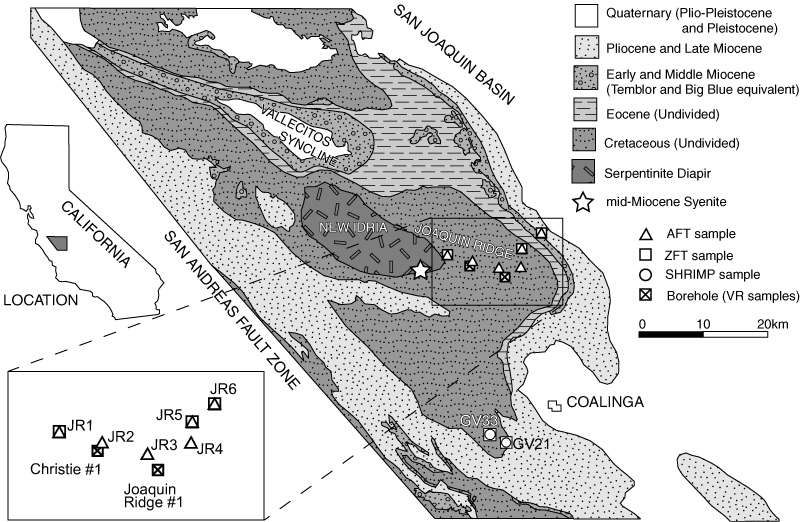
\includegraphics[width=600pt]{geomapBate_small.jpg}
  \caption{ 
 Simplified geologic map of the  Great Valley Group near Coalinga with
 the sample locations.  Modified from  Bate (1985).}\label{fig:gvgeology}
  \end{center}
  \end{figure}

This paper focuses  on samples of the Great  Valley Group collected in
and around  Joaquin Ridge near  Coalinga (Figure \ref{fig:gvgeology}).
These  sedimentary  rocks  contain geochronological  and  petrographic
information about  the evolution of their source  region, the Mesozoic
Sierra  Nevada magmatic  arc.   They also  contain  clues about  their
post-depositional history,  and the  tectonic evolution of  the Diablo
Range  in  which  they  are now  exposed.   Conventional  petrographic
studies  of Great  Valley Group  rocks indicate  that, with  time, the
lithic fraction  of the sediments  decreased, the percentage  of total
feldspar increased  and the composition  of the feldspars  became more
potassic.   These trends  reflect increasing  chemical  and geomorphic
maturity of  the magmatic arc (Ingersoll,  1979, 1983).  Paleocurrents
are  dominantly  west-directed, indicating  that  the  source was  the
southern Sierra Nevada (Ingersoll, 1979).  In addition to conventional
petrographic studies, samples in the vicinity of Coalinga were studied
by bulk-rock  $\epsilon_{Nd}$ and $\epsilon_{Sr}$  analysis (Linn {\it
et al.},  1991, 1992),  confirming the petrographic  results.  Between
Cenomanian  and  Maastrichtian  time,  $\epsilon_{Nd}$  systematically
decreased from -0.7  to -5.0 (Linn {\it et  al.}, 1991), reflecting an
eastward migration of the drainage divide, to where the Sierran magmas
are more  continental in  composition (De Paolo,  1981).  Some  of the
samples of  Linn {\it et  al.}  (1991) were used  by DeGraaff-Surpless
{\it  et  al.}   (2002)  for  SHRIMP  single  grain  zircon  U/Pb  age
measurements, which  confirmed that the sediment source  for the Great
Valley Group in the San  Joaquin Valley is the southern Sierra Nevada,
as the  most frequently observed ages  are 102-132 Ma.   The spread of
the Mesozoic ages and the  number of peaks in the grain-age histograms
increase  with  decreasing  depositional  age.  This  may  reflect  an
expansion of  fluvial drainage basins, resulting in  a larger sediment
source  area.   The  minimum   lag-time  between  the  age  of  zircon
crystallization and  deposition (determined by  paleontology) is short
(3-15 Ma).  This constrains the Late Cretaceous exhumation rate of the
Sierra  Nevada (Surpless, 2001)  -- constraints  that this  paper will
attempt to refine.  \\

Nevertheless,  considerable controversy  exists  about the  exhumation
history of  the Sierra  Nevada batholith. Some  workers, based  on the
observation of  uplifted and tilted Cenozoic strata,  believe that the
development of  Sierran topography occurred  in the last 10  My (e.g.,
Unruh, 1991).  Others claim  that significant topography existed since
at least the Early Cenozoic based on old (U-Th)/He cooling ages of the
Sierra Nevada granites, and the  fact that the spatial distribution of
these ages  preserves the signature  of old topography (House  {\it et
al.}, 1998,  2001).  Both opinions  are based upon data  acquired from
rocks  of  the modern  Sierra  Nevada. They  seldom  make  use of  the
continuous record  of sediments shed  from the ancient  mountain range
since the Late Jurassic.   These sediments are excellent ``witnesses''
of the evolution  of the Sierra Nevada, for much  of the batholith and
its volcanic carapace have long since been removed.\\

Detritus  from the  Sierra Nevada  was deposited  in the  Great Valley
forearc  basin.    Above  these  strata  was   deposited  a  gradually
shoaling-upward  succession  of   Cenozoic  deposits  (Dibblee,  1971;
Bartow, 1991).  A total thickness  of 6000-8000m of the Upper Jurassic
through Cretaceous Great Valley Group is exposed in a homocline on the
eastern flanks of the Diablo Range (Dickinson, 2002).  Superimposed on
this  homocline  are  folds   formed  as  a  result  of  right-lateral
transpressional  strike-slip deformation along  the San  Andreas fault
(Miller,  1998).  The Vallecitos  syncline is  one of  these synclinal
folds (Figure \ref{fig:gvgeology}). Cenozoic strata contain petroleum,
although  they  are  buried  less  than 1500m  deep  in  the  syncline
(Rentschler, 1985).  The heat  source for oil generation is enigmatic.
Joaquin Ridge forms the anticline adjacent to the Vallecitos syncline.
The  New  Idria serpentinite  body  is exposed  in  the  core of  this
anticline.   A  few  small  intrusions  of syenite  crop  out  in  the
serpentinite body, and are dated at $\sim$12.8 Ma (no error stated) by
$^{40}$Ar/$^{39}$Ar  dating on  the amphibole  barkevikite (Obradovich
{\it  et al.},  2000). Rb-Sr  dating of  benitoite yielded  an  age of
$\sim$ 12 Ma  (no error stated) (Obradovich {\it  et al.}, 2000).  The
Mendocino  triple  junction  passed  the  latitude  of  New  Idria  at
$\sim$12-14 Ma (Johnson  and O'Neill, 1984).  $\sim$14 Ma  is also the
age  of the  spectacular deposits  of  the Big  Blue Formation,  which
consist   almost  solely  of   sedimentary  serpentinite   (Casey  and
Dickinson, 1976; Bate, 1985).\\

In the following sections, new fission track and vitrinite reflectance
data are presented, followed by  a discussion of implications of these
data.  To reconstruct the  pre-depositional history of sediments, they
must not be thermally reset.  Therefore, the post-depositional history
of  the  New  Idria  area   will  be  discussed  first.   Among  other
conclusions  we demonstrate that,  until the  rapid exhumation  of the
serpentinite  dome,  this  area   was  characterized  by  low  thermal
gradients that  prevented the buried sediments from  being heated very
much.  The  discussion of  the pre-depositional history  then follows.
This  paper  illustrates  the  great  power  of  simultaneously  using
multiple  thermochronometers on  detrital  sediments. Each  individual
thermochronometer  only tells  part of  the  story, but  the whole  is
greater  than the  sum of  the parts.   When all  evidence  is jointly
considered, a self-consistent story  emerges that traces the sediments
from their  crystallization in the Cretaceous Sierra  Nevada until the
final stages  of their  exhumation on Joaquin  Ridge.  This  story not
only  has consequences for  the regional  geology of  the Coalinga/New
Idria area, but also for the tectonic history of the Sierra Nevada and
the petroleum geology of the Vallecitos syncline.

\section*{\uppercase{Methods}}

Figure  1 shows  a  simplified geologic  map  of the  field area  with
indication  of  the sample  locations.   Some  of  these samples  were
previously  discussed   by  Linn  {\it  et  al.}    (1991,  1992)  and
DeGraaff-Surpless  {\it et al.}   (2002).  They  are labeled  with the
letters  ``GV''.  An  additional six  samples were  collected  along a
transect on  Joaquin Ridge  and are labeled  with the  letters ``JR''.
Table   \ref{tab:summary}   summarizes   the  geochronological   data.
Apatites and  zircons were  separated from their  host rock  using the
mineral  separation techniques reported  by DeGraaff-Surpless  {\it et
al.}   (2002).  All  samples  yielded abundant  euhedral apatites  and
zircons.   Both zircon and  apatite fission  track ages  were measured
with  the  external detector  method  (e.g.,  Dumitru, 2000).   Figure
\ref{fig:AFTages} shows  the apatite  fission track data  from Joaquin
Ridge, arranged in order of decreasing stratigraphic age.  Five of six
samples on Joaquin  Ridge came from the Great  Valley Group, while the
youngest sample (JR6) came  from the Middle  Miocene Temblor Formation,
beneath   the    Middle    Miocene   Big    Blue   Formation.    Figure
\ref{fig:ZFTages} shows five zircon  fission track samples labeled and
arranged  in decreasing order  of stratigraphic  age like  the apatite
fission track  ages of Figure \ref{fig:AFTages}.  The  dark gray bands
on  the radial  plots  of samples  GV21  and GV33  mark  the range  of
crystallization ages measured by U/Pb SHRIMP dating (DeGraaff-Surpless
{\it et al.}, 2002).  The  light gray bands mark the depositional ages
(Dibblee, 1971). Between  n=20 and n=41 grains were  dated per fission
track sample. The probability p that either the oldest or the youngest
population fraction of size f was missed by all n grains is given by:

$$p  = 2(1-f)^n - (1-2f)^n$$

For example, if n=30 and f=0.12,  then p=5\%. In other words, there is
5\% chance that either the youngest or the oldest 12\% of the detrital
population  was  missed. In  addition  to  the aforementioned  outcrop
samples, we also had access  to material from two boreholes on Joaquin
Ridge, the ARCO ``Christie \#1'' and ARCO ``Joaquin Ridge \#1'' wells.
Vitrinite reflectance  measurements were performed on  23 well cutting
samples  from  ``Joaquin  Ridge  \#1''  and three  core  samples  from
``Christie \#1''.  Up  to 100 reflected light points  were measured on
the  vitrinite populations  represented  in each  sample.  The  lowest
reflectance values likely reflect contamination from organic matter in
the drilling  fluid, while some  of the higher reflectance  values may
represent  resedimented vitrinite.   However, rather  than arbitrarily
rejecting some  data, we have opted  to just contour and  plot all the
data (Figure \ref{fig:vitrinite}).  The  raw data for both the fission
track and the vitrinite reflectance analysis are available in the Data
Repository \footnote[1]{Data Repository item 2005xxx}.


\begin{table}[htbp]
  \centering
\begin{tabular}{c|ccccc}
sample & location & depo age & U/Pb age & ZFT age & AFT age\\
name & (lat/lon) & (Ma) & (Ma) & (Ma) & (Ma)\\
\hline
      GV33 & 36$^o$6'/120$^o$27' & 89-95 & 131$\pm$5 &  100$\pm$6.5 & \\
      GV21 & 36$^o$5'/120$^o$25' & 81-87 & 132$\pm$4 & 98.7$\pm$4.4 & \\
       JR1 & 36$^o$20'/120$^o$31.5' & 90-100 & & 98.1$\pm$4.3 & 13.3$\pm$0.9 \\
       JR2 & 36$^o$19'/120$^o$35' & 90-93.5 & & & 71.9$\pm$3.2 \\
       JR3 & 36$^o$18.5'/120$^o$26.5' & 78-83.5 & & & 84.3$\pm$3.3 \\
       JR4 & 36$^o$20'/120$^o$24' & 71.3-75 & & & 80.9$\pm$2.8 \\
       JR5 & 36$^o$19'/120$^o$24' & 66-68 & & 89.2$\pm$4.5 & 81.5$\pm$3.8 \\
       JR6 & 36$^o$15.5'/120$^o$23' & 16.4-14.8 & & 13.1$\pm$1 \& & 17.0$\pm$3 \& \\
           & & & & 84.3$\pm$16 (*) & 49.7$\pm$6 (*) \\
\end{tabular}
  \caption{
Summary table  of geochronological data. U/Pb dating  was performed on
zircon  and fission  track dating  on  both zircon  (ZFT) and  apatite
(AFT). All fission  track ages are central ages  (Galbraith and Green,
1993) except for  JR6 (*),  for which the  two best  fitting component
ages are  reported, calculated with the binomial  peak fitting routine
of Brandon (1996).}
  \label{tab:summary}
\end{table}

\section*{\uppercase{Discussion}}

\subsection*{Fission track data}
\label{sec:FT}

Apatite  fission  tracks  are  immediately  annealed  at  temperatures
$>\sim$110$^o$C  (e.g.,   Wagner  and   Van  den  Haute,   1992).   At
temperatures  less  than about  60$^o$C,  apatite  fission tracks  are
completely  preserved.   The  temperature  zone between  $\sim$60  and
$\sim$110$^o$C  is  named  the  apatite  fission  track  {\it  partial
annealing zone}  (e.g., Dumitru, 2000).  In this  zone, fission tracks
are not  immediately annealed, but gradually shortened  with time. The
annealing temperature of zircon  fission tracks is more controversial,
but  generally  considered  to  lie  between  230  and  310$^o$C  (see
discussion by Tagami and Dumitru, 1996). In this paper, we will assume
the more ``conservative'' value of $\sim$230$^o$C.\\

\begin{figure}[here]
  \centering
  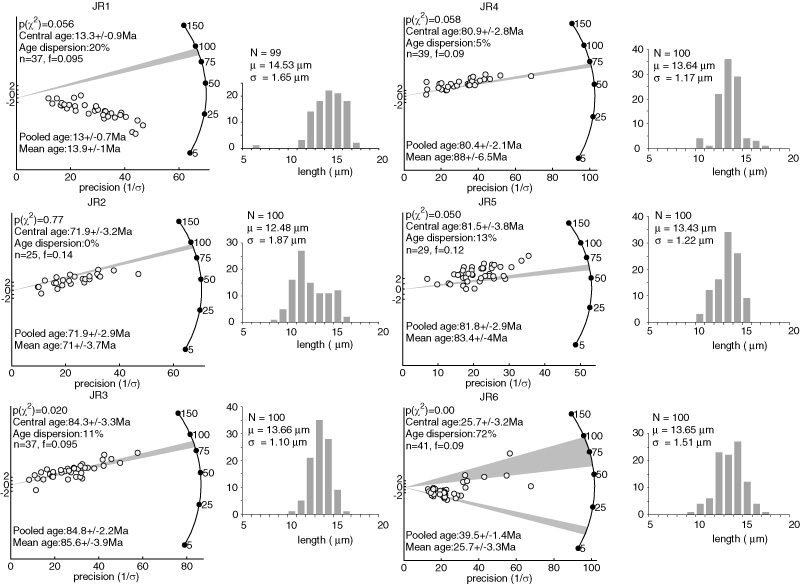
\includegraphics[width=400pt]{AFT.jpg}
  \caption{
Apatite fission  track radial plots  (Galbraith, 1990) of  the Joaquin
Ridge.  The  gray bands  represent depositional ages.   The histograms
show the fission track length distributions. n = number of grains, f =
largest  population fraction  of older/younger  grains that  are p=5\%
likely to have been missed, N = number of confined tracks.}
\label{fig:AFTages}
\end{figure}

First,  we  will  discuss  the  apatite  fission  track  data  (Figure
\ref{fig:AFTages}). Of the five  Great Valley Group samples, four have
exclusively  Cretaceous apatite  fission track  grain-ages, indicating
that  these grains  never reached  temperatures greater  than 110$^o$C
since their deposition in the Great Valley Group.  However, sample JR2
has the oldest depositional age of these four samples but the youngest
fission track ages,  with the latter being even  slightly younger than
the  former.   Therefore,  JR2  has  been  partially  reset,  and  saw
temperatures less  than $\sim$110$^o$C, but  well above $\sim$60$^o$C.
The fission tracks  of sample JR2 are also  significantly shorter than
those of  the other  samples, an additional  suggestion that  JR2 must
have been  heated to well  within the partial annealing  zone.  Sample
JR1, located the  nearest to the New Idria  serpentite, has completely
annealed  apatite  fission tracks  and,  therefore,  was heated  above
$\sim$ 110$^o$C.   It dates the end  of the heating  event at $\sim$14
Ma.  Sample  JR6 from the  Miocene Temblor Formation contains  two age
components:   one  Cretaceous   and  one   Miocene   component  (Table
\ref{tab:summary}).  There also is a hint of bimodality in the fission
track  length  distribution.   A   first  group  of  relatively  short
($\sim$9-13 $\mu$m)  fission tracks  formed prior to  the mid-Miocene.
These  tracks  preserve Sierran  provenance  ages  but were  partially
annealed during the mid-Miocene thermal event.  A second group of long
fission tracks  ($\sim$13-17 $\mu$m) formed after  this thermal event,
and have not been annealed since then.  Paleocurrent directions in the
Temblor  and  Big  Blue  Formations  are west-to-east,  which  is  the
opposite  flow direction  as for  the  Great Valley  Group (Casey  and
Dickinson,  1976; Bate,  1985;  Bent, 1985).   Therefore, the  apatite
grains  of  the  Temblor  Formation  have been  redeposited  from  the
underlying Great  Valley Group, some  of which was  thermally annealed
during a mid-Miocene thermal event.\\

\begin{figure}[here]
  \centering
  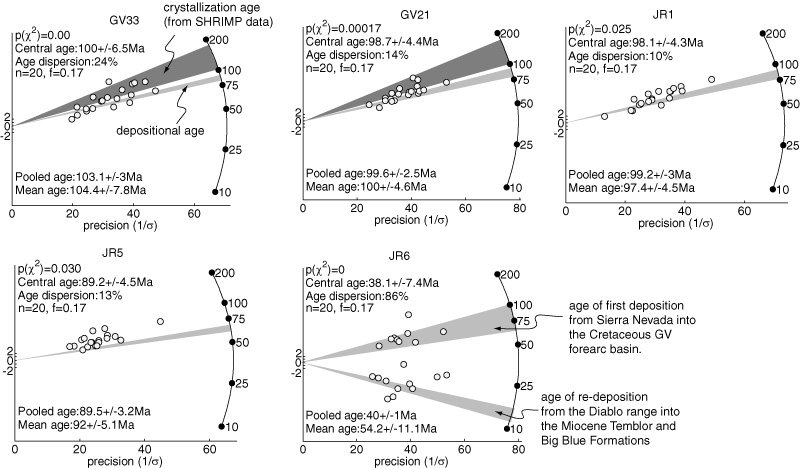
\includegraphics[width=400pt]{ZFT.jpg}
  \caption{
Zircon fission  track radial  plots.  As in  Figure \ref{fig:AFTages},
the light gray bands represent depositional ages.  The dark gray bands
mark the  crystallization ages, as measured  by DeGraaff-Surpless {\it
et al.}  (2002) using the U/Pb method  on zircon. n and f as in Figure
\ref{fig:AFTages}.}
  \label{fig:ZFTages}
\end{figure}

The zircon fission  track ages for four of the  five samples are older
than   the   age   of    Great   Valley   Group   deposition   (Figure
\ref{fig:ZFTages}).  Sample JR1, which had completely annealed apatite
fission  tracks,   also  has   unreset  zircon  fission   track  ages.
Therefore, sample JR1 was heated to more than $\sim$110$^o$C, but less
than   $\sim$230$^o$C   after  its   deposition.    The  lag   between
crystallization,  exhumation and  deposition times  were  short, which
means that  the source area  of these sediments exhumed  rapidly.  The
most  surprising observation is  that the  Middle  Miocene  sample JR6,
which had a bimodal apatite fission track age distribution, also has a
bimodal zircon fission track distribution. The oldest mode of Mesozoic
ages is compatible with the  unreset fission track ages of the Joaquin
Ridge  samples   located  away  from  the   serpentinite  body  (Table
\ref{tab:summary}).   The youngest  age  peak is  concordant with  the
$\sim$14  Ma apatite fission  track age  of sample  JR1, and  with the
youngest mode  of the apatite  fission track age distribution  of JR6.
Because not all  the apatite grains in JR6 were  reset at $\sim$14 Ma,
we know that  this sample was not heated  to more than $\sim$110$^o$C.
In fact,  there is ample evidence  that the Temblor  formation did not
see temperatures higher than  $\sim$56$^o$C east of Joaquin Ridge (see
below). Therefore,  the $\sim$14  Ma old zircons  must have  been been
annealed prior to  deposition in the Temblor and  Big Blue formations.
Recalling the eastward paleocurrents of these deposits, this indicates
that at least  part of the provenance area  for the Temblor Formation,
which   is   Joaquin   Ridge,   reached  temperatures   as   high   as
$\sim$230$^o$C as recently as $\sim$14 Ma.

\subsection*{Vitrinite reflectance data}

\begin{figure}[here]
  \centering
  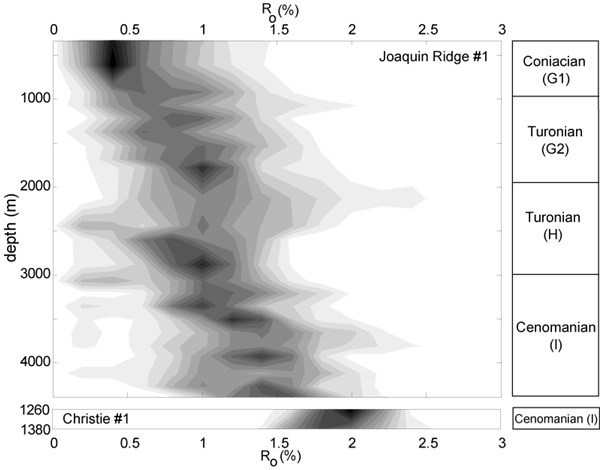
\includegraphics[width=400pt]{Vitrinite.jpg}
  \caption{
  Contoured  vitrinite reflectance  results for  two wells  on Joaquin
  Ridge (for their location, see Figure~\ref{fig:gvgeology}).}
  \label{fig:vitrinite}
\end{figure}

Additional  evidence   for  a  heating  event   comes  from  vitrinite
reflectance   data   from   two    wells   on   Joaquin   Ridge   (see
Figure~\ref{fig:gvgeology}  for   the  location  of   the  wells,  and
Figure~\ref{fig:vitrinite} for  the vitrinite reflectance  data).  The
``Joaquin Ridge \#1'' well is 4,390 m deep and located in the vicinity
of sample JR3.  The ``Christie \#1'' well is 1,380 m deep, and located
next to sample JR2.  Micro-paleontological ages have been obtained for
both wells (Martin B.  Lagoe, written communication).  ``Joaquin Ridge
\#1'' sediments are of Coniacian (at 910 m) to Cenomanian age (at TD),
whereas  the ``Christie  \#1'' samples  at TD  are  Cenomanian (Figure
\ref{fig:vitrinite}).  Twenty-three  samples from the  ``Joaquin Ridge
\#1'' well  were analyzed, from depths  of 300 to 4,390  m.  They show
$R_o$  values  of  0.6-1.5\%,  explaining why  apatite  fission  track
samples  JR3, JR4,  and  JR5  have not  been  thermally reset.   These
samples are all located  upsection from the shallowest ``Joaquin Ridge
\#1'' vitrinite reflectance  samples and should, therefore, correspond
to  $R_o$ values $<$  0.6\%, or  maximum paleo-temperatures  less than
$\sim$85$^oC$ (Sweeney and Burnham,  1990).  The ``Joaquin Ridge \#1''
vitrinite  reflectance  data  imply  a thermal  gradient  of  $\sim$14
$^o$C/km, which was normal in the Great Valley forearc basin (Dumitru,
1988).  There exists substantial evidence that the geothermal gradient
in the Great  Valley Group was very low during  the Cretaceous and the
beginning of the Tertiary.  This  is postulated to have been caused by
the refrigerating  effect of  the subducting Farallon  pLate (Dumitru,
1988).  The ``Christie  \#1'' well is located near  sample JR2.  Three
cores taken in ``Christie \#1''  at 1,250-1,380 m are characterized by
vitrinite   reflectance   values   of  $\sim$1.9-2.0\%,   or   maximum
paleotemperatures  of $\sim$180$^oC$,  very hot  for the  Great Valley
Group.   However,  apatite fission  track  sample  JR2, located  about
1,500-2,000   m  upsection   from  the   ``Christie   \#1''  vitrinite
reflectance samples, has not  been reset.  Assuming a thermal gradient
similar to  that inferred  from the ``Joaquin  Ridge \#1''  well, this
would lower  the predicted vitrinite reflectance value  for sample JR2
to  about $R_o$  = 1.3\%  (maximum  paleo-temperature $\sim$150$^oC$).
This rough  estimate, if correct, conflicts with  the observation that
apatite  fission track sample  JR2 has  not been  completely annealed.
This would  imply that the high  $R_o$ values of  ``Christie \#1'' are
due to a  thermal anomaly, that the thermal gradient  in this well was
not equal to that of  ``Joaquin Ridge \#1'', and/or that this gradient
was  not  linear.   Although  not   reset,  sample  JR2  has  been  at
paleo-temperatures above those of samples JR3, JR4, and JR5.  The high
paleo-temperatures of the ``Christie  \#1'' samples are unlikely to be
the result  of simple  burial, but are  instead interpreted to  be the
result of a  Middle  Miocene heating spike, associated  with the upward
protrusion and tectonic denudation of the New Idria serpentinite body.

\section*{\uppercase{Implications for the post-depositional history of the Great Valley Group}}

Partial  annealing of apatite  fission track  sample JR2  and complete
annealing of  JR1 at  $\sim$14 Ma by  burial-induced heating  alone is
improbable for at least two reasons:

\begin{itemize}
\item Maximum temperatures of the  Great Valley Group on Joaquin Ridge
did not  coincide with the timing  of maximum burial.   In the Panoche
Hills  area, north of  Joaquin Ridge,  subaerial exposure  and erosion
occured  intermittently  in  the  Paleocene  and  Eocene,  and  almost
continuously  since   the  Oligocene  (Moxon,   1990;  Bartow,  1991).
Furthermore, deposits  as old as  the Eocene Kreyenhagen  Formation of
Oil Canyon,  10 kilometers north of Coalinga,  contain biogenic silica
in the form  of opal-A (Milam, 1985), indicating  that they were never
heated  above  28-56$^oC$  (Murata   and  Larson,  1975).   The  total
thickness of  Tertiary deposits presently  outcropping at the  nose of
Joaquin Ridge is only $\sim$1.5 km (Dibblee, 1971).
\item  The age  of  the annealing  (as  dated by  sample JR1)  exactly
coincides  with the exhumation  of the  nearby New  Idria serpentinite
body (see the  next paragraphs). It is unlikely  that this coincidence
is mere chance.
\end{itemize}

An alternative  explanation for the vitrinite  reflectance and fission
track  data  is  that  the  Great  Valley  Group  was  heated  by  the
serpentinite  diapir.   Three  lines  of  evidence  suggest  that  the
serpentinite  body  was  hot  when  it  breached  the  surface.   Most
importantly,  mineral  assemblages  of  Franciscan inclusions  in  the
serpentinite  body indicate that  it rose  from depths  of as  much as
$\sim$20 km which, even under the lowest thermal gradients, would make
them  relatively  hot  ($>$200$^o$C;  Coleman, 1996).   Secondly,  the
serpentinite diapir  rose very rapidly. Evidence for  the massive size
and sudden nature of this event is contained in the Middle  Miocene Big
Blue Formation, which  crops out $\sim$15 km east  of the serpentinite
dome.  The Big Blue Formation consists almost entirely of serpentinite
clasts,  some of  which  are house-sized  (Anderson  and Pack,  1915).
Paleocurrents  indicate  flow  towards   the  east,  in  the  opposite
direction of  the ``normal''  Great Valley Group  paleocurrents (Casey
and Dickinson,  1976; Bate, 1985).   The facies gradient  from sheared
protrusive  serpentinite  through braided  stream  deposits to  marine
tidal flat facies evinces  an eastward facing paleoslope (Bate, 1985).
The  fluvial  deposits preserving  paleocurrents  were  shed from  the
gradually spreading flank of  a New Idria serpentinite protrusion that
breached the suface to form  a dome-like mass that spread laterally as
additional serpentinite was supplied to the surface by upward diapiric
flowage from within  the crust.  If the serpentinite  body rose to the
surface extremely rapidly, it is  likely to have remained hot all that
time.  Finally, serpentinization reactions are {\it exothermic}:\\

Antigorite:
$\rm 34 Mg_2SiO_4 + 51   H_2O \rightarrow Mg_{48}Si_{34}O_{85}(OH)_{62} + 20Mg(OH)_2$\\

Chrysotile:
$\rm 2 Mg_2SiO_4 + 3 H_2O \rightarrow Mg_3Si_2O_5(OH)_4 + Mg(OH)_2$\\

Both of  these reactions require  a lot of  water.  This could  be the
reason  why the  serpentinization  did not  happen  before the  Middle 
Miocene.   At that  time,  the Mendocino  triple  junction passed  the
latitude  of Coalinga.   The faulting  and folding  caused by  the San
Andreas  fault might  have  introduced  a pathway  for  fluids in  the
ophiolitic  crust that  underlies the  Great Valley  Group.   Both the
reaction enthalpy $\Delta H$ of the serpentinization reactions and the
heat capacity C$_p$ of the serpentinite minerals vary with temperature
(Holland  and Powell,  1998). At  the conditions  relevant to  the New
Idria serpentinite dome, the pressure effect is negligible. Making the
simplifying  assumption  that  serpentinization  of  the  entire  body
occurred   at  the  same   time,  we   can  calcuLate   a  first-order
approximation of the maximum temperature increase that could be caused
by the serpentinization:

$$\rm \Delta T = \frac{\Delta H}{C_p}$$

\begin{figure}[here]
  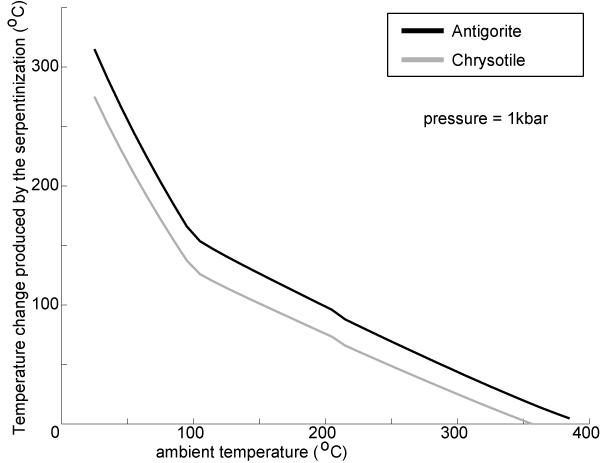
\includegraphics[width=0.6\textwidth]{serpentinization.jpg}
  \caption{
  Serpentinization  reactions  are  less  exothermic  as  the  ambient
  temperature increases.   The New  Idria serpentinite body  must have
  been relatively hot for one of two reasons: (1) it formed under high
  ambient temperatures, or (2) it generated the heat itself.}
\label{fig:serpentinization}
\end{figure}

The evolution  of this reaction  temperature as a function  of ambient
temperature is shown  in Figure \ref{fig:serpentinization}.  The lower
the  ambient  temperature, the  more  exothermic the  serpentinization
reactions are, but  above a few hundred degrees,  they can even become
endothermic.   The buffering  thermodynamics  of the  serpentinization
reactions are such that the  serpentinite body must have been hot when
it formed, either because the  ambient temperature was high or because
of its own reaction heat.  A rough estimate of the thermal effect that
a hot, spherical  body the size of the New Idria  diapir would have on
the adjacent country rock can be calculated assuming simple conductive
cooling:

$$ T(r,t) = \frac{T_i}{2} \left(erf\left
            (\frac{R-r}{2 \sqrt{\kappa t}}\right)
            + erf\left(\frac{R+r}{2 \sqrt{\kappa t}}\right)\right) 
         + T_i \frac{\sqrt{\kappa t}}{r \sqrt{\pi}} 
          \left(exp\left(-\frac{(r+R)^2}{4 \kappa t}\right)
              - exp\left(-\frac{(r-R)^2}{4 \kappa t}\right)\right)$$

with $T_i$ the initial temperature difference between the serpentinite
and the country  rock, R the radius of the  sphere ($\sim$10km), r the
distance  from the  center  of the  sphere,  $\kappa$ the  diffusivity
($\sim 10^{-6}$m$^2$/s), and t time (modified from Carslaw and Jaeger,
1959).   Figure  \ref{fig:thermalmodel}   shows  the  result  of  this
calculation.  It  indicates that  during $\sim$10$^6$ years  after the
intrusion of  a hot body the size  of the New Idria  diapir, the rocks
within a  few km of the  contact would experience  a transient heating
spike.  Added to the pre-existing background geothermal gradient, this
spike  could  explain both  the  vitrinite  reflectance  data and  the
apatite  fission  track  annealing  behavior.   Thermal  halos  around
protrusive  serpentinite bodies of  west-central California  have been
described by Murata  {\it et al.}  (1979), who  traced the Marca Shale
Member  of the  Upper  Cretaceous and  Paleocene petroliferous  Moreno
Shale over a distance of 120 km and found that biogenic silica in this
unit was  cristobalitic everywhere, except  for the northern  flank of
Joaquin Ridge, where  it comes within less than 1 km  of the New Idria
serpentinite body.  This is the  only place where  quartz-phase silica
exists, indicating maximum temperatures $> \sim 80^o$C.\\

\begin{figure}[here]
  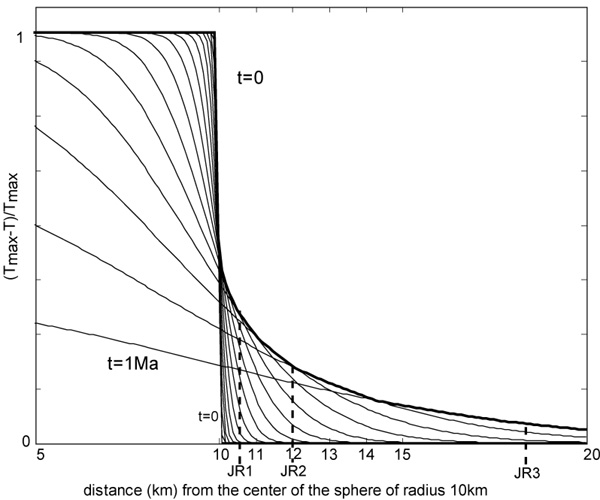
\includegraphics[width=400pt]{thermalmodel.jpg}
  \caption{
Conductive cooling  of a  hot sphere surrounded  by a  cooler material
creates  a transient  heating signal  in the  latter.  Let  the sphere
(radius  = 10km,  left side  of the  figure) represent  the  New Idria
serpentinite body, rapidly rising in a Great Valley Group country rock
(right  side  of  the  figure)  with thermal  diffusivity  $\kappa$  =
10$^{-6}$ m$^2$/s. Then  the thin black lines show  the evolution with
time (from  0 to 1Ma)  of the thermal  contact.  The thick  black line
connects the maximum temperatures  reached at different distances. The
location of three  of the fission track samples is  also marked on the
figure.}
\label{fig:thermalmodel}
\end{figure}

We  have not attempted  to rigorously  model petroleum  generation and
trapping in the Vallecitos syncline, but current studies by the United
States Geological  Survey may  better constrain the  petroleum history
(Peters {\it  et al.}, 2005). Nevertheless,  various relations provide
general constraints on petroleum generation and accumulation, and thus
provide  a point  of  comparison for  our interpretation.   Biomarkers
recently collected from the Vallecitos  oil field by the United States
Geological Survey  show biomarker and  isotope compositions indicative
of  Upper  Eocene  Kreyenhagen  source rocks  (written  communication,
Kenneth E.  Peters).   However, the small pools in  the syncline occur
mainly  in  fault  traps   located  under  the  Kreyenhagen  Formation
(California  Division   of  Oil   and  Gas,  1982).    Therefore,  the
Maastrichtian-Danian Moreno Formation might be a more plausible source
of these  hydrocarbons.  Although not understood in  detail, the fault
traps likely  developed when  the syncline folded  in the  Late Middle 
Miocene (Rentschler, 1985). Thus, maturation, migration and entrapment
likely occured no earlier than  Late Miocene, consistent with our data
and interpretation.\\

\section*{\uppercase{Implications for the Cretaceous history of the Sierra Nevada}}
\label{sec:predepo}

Most  geochronological  methods   have  a  {\it  closure  temperature}
(Dodson,  1973).  However,  in the  apatite fission  track  method for
example, there is  not one distinct temperature, but  a rather diffuse
zone over which the geochronological system ``closes''.  Nevertheless,
for our purposes, the rather crude concept of a closure temperature is
still useful.  For the U/Pb  system in zircon, the closure temperature
is as high at $\sim$900$^oC$  (Dahl, 1997; Miller {\it et al.}, 2003).
The  closure  temperature  of  the  zircon  fission  track  method  is
somewhere between  $\sim$230 and 310$^o$C  (Wagner and Van  den Haute,
1992;  Tagami  and Dumitru,  1996).   For  the  apatite fission  track
method, a closure temperature  of $\sim$100$^o$C can be used, although
this  value varies with  apatite chemistry  (e.g., Gleadow  and Duddy,
1981).\\

A frequent  practice in igneous  and metamorphic geochronology  is the
simultaneous use of  several dating techniques on the  same sample.  A
graph  of apparent  age versus  closure  temperature is  then used  to
estimate  the cooling  history of  such  a sample  (e.g., Harrison  and
McDougall,  1980).   A  similar  approach  can be  used  for  detrital
samples.  Conservatively assuming that the  tops of the plutons in the
southern  Sierra  Nevada  were  emplaced  at  2-3km  depth  (Ague  and
Brimhall,  1988), Surpless  (2001) argued  argued that  the relatively
short  minimum  lag  times  between  the  U/Pb  zircon  ages  and  the
depositional  ages  of  3-15Ma   indicated  rapid  exhumation  of  the
Cretaceous Sierra Nevada at rates  of $\sim$ 0.6-1mm/yr. We can extend
this  method  to the  lower  temperature  thermochronometers of  Table
\ref{tab:summary}.\\

If  we had  access to  double-dated grains,  as in  Rahl {\it  et al.}
(2003), estimating the  probability distribution of provenance cooling
rates  would   be  a  trivial  exercise.   However,   because  of  the
uncontroversial  provenance  of our  samples  and  the  fact that  the
southern Sierra Nevada  can be considered a structurally  more or less
homogeneous  fault block,  we might  be able  to proceed  without such
data. Thus, we can get a  first order estimate of the cooling rates by
looking at  the time  lag between  the mean (or  central) ages  of two
thermochronological grain-age  populations (e.g.,  ZFT and AFT),  or at
that between the  mean (or central) age of  a grain-age population and
the depositional age of the sample.\\

Doing this  for the thermally unreset data  of Table \ref{tab:summary}
yields seven apparent  cooling rates which do not  show any systematic
variation with depositional age.  The weighted mean of these estimates
yields an apparent cooling  rate of $\sim$21$^o$C/Ma. Depending on the
thermal  gradient (22-40$^o$C/km; Rothstein  and Manning,  2003), this
then corresponds to exhumation rates of $\sim$0.5-1mm/yr, which agrees
with the  estimates of Surpless  (2001) and Ague and  Brimhall (1988).
These are rather high rates, but this does not come as a surprise when
we consider the amount of sediment deposited in the Great Valley Group
at the time.

\section*{\uppercase{Summary and conclusions}}

\begin{figure}[here]
   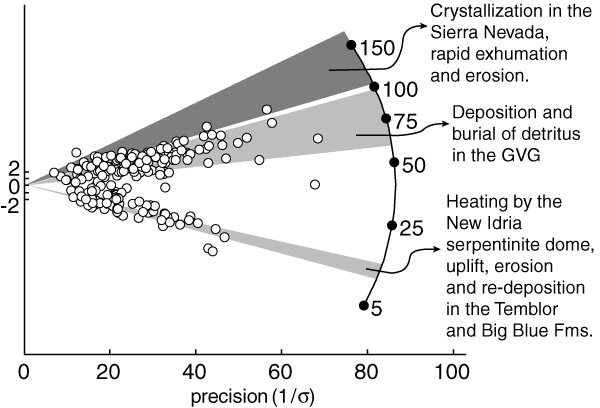
\includegraphics[width=400pt]{compiledAFT.jpg}
   \caption{
The history of Joaquin Ridge  sediments summarized on a single fission
track radial plot, compiled from all the apatite fission track data.}
   \label{fig:JR6}
\end{figure}

Figure \ref{fig:JR6} summarizes the  history of the Great Valley Group
near Coalinga and New Idria:
\begin{itemize}
\item  The U/Pb,  zircon and  apatite  fission track  ages of  unreset
 apatite  and zircon show  that the  southern Sierra  Nevada underwent
 rapid  and steady  exhumation  during the  Late  Cretaceous.  As  the
 exhuming mountain  range was eroded,  it shed sediments in  the Great
 Valley  forearc basin.  These  sediments are  presently exposed  in a
 homocline on the eastern flank of the Diablo Range.
\item The Great  Valley Group turbidites were buried  to great depths,
 but  under  refrigerated thermal  gradients,  produced by  Franciscan
 subduction (Dumitru, 1988).
\item  During  the  Middle   to  Late  Miocene  ($\sim$12-14  Ma),  the
 Mendocino triple junction migrated from south to north to the west of
 Coalinga (Johnson and O'Neil, 1984).  Its passage was associated with
 minor igneous  activity, dated at  $\sim$12.8 Ma (Obradovich  {\it et
 al.}, 2000).
\item  The  faulting and  folding  caused  by  the San  Andreas  fault
 introduced fluids  in the ophiolitic  crust that underlies  the Great
 Valley Group.   These fluids reacted  with the peridotitic  rocks and
 formed  serpentine  minerals. Because  of  its  low  density and  the
 relative  ease with  which it  deformed, the  serpentinite  body rose
 rapidly.   The combined effect  of the  folding and  the rise  of the
 serpentinite diapir  caused substantial uplift of  Joaquin Ridge, and
 secondary folding  and faulting  in the adjacent  Vallecitos Syncline
 (Rentschler,   1985).     Paleocurrent   directions   reversed,   and
 re-sedimentation  of Great  Valley Group  detritus formed  the Middle
 Miocene Temblor  and younger  formations.  The Big  Blue came  to the
 surface as a rising hot protrusion, heating the Great Valley Group on
 the way up and spreading at once over the countryside.
\item Because it formed at great depth or because the serpentinization
 reactions  are exothermic, the  New Idria  serpentinite body  was hot
 when it approached the surface,  forming a thermal halo.  The heating
 was  sufficient  to completely  anneal  apatites  in the  surrounding
 country rock  and explain  the relatively high  vitrinite reflectance
 values that  are observed near  the contact between the  Great Valley
 Group and the serpentinite body.
\item  The  heat  released  by the  serpentinite  produced  diagenetic
 alteration of cristobalitic to  quartzose silica in the Moreno Shale,
 which underlies the Vallecitos  syncline (Murata {\it et al.}, 1979),
 pushing the source rocks of this basin into the thermal oil window.
\item Alternatively,  it is possible  that syenitic intrusions  in the
 serpentinite body provided the  ``missing'' heat source.  However, we
 think  that  the  serpentinite   body  itself  is  a  more  realistic
 alternative  because   it  is  size  rather   than  temperature  that
 determines the  amount of time it takes  for a hot body  to cool, and
 the size of the resulting thermal halo. A small igneous intrusion may
 have been hotter  than the serpentinite protrusion, but  it would not
 be felt as long, and as far into the country rock.
\item  Deformation and  folding  continue in  the  Joaquin Ridge  area
 today, witnessed  by the 1983 Coalinga  earthquake.  However, gravity
 data suggesting  that the root  of the New  Idria body is only  a few
 kilometers deep, imply that the exhumation of the serpentinite diapir
 has almost stopped (Byerly, 1966; Casey and Dickinson, 1976).
\end{itemize}

\section*{\uppercase{Acknowledgements}}

This  research  was  partly  funded  by  GSA  student  research  grant
\#7298-02 to Pieter Vermeesch.  Well cuttings were provided by William
Bazeley and ARCO Inc.  Vitrinite reflectance analysis was performed by
Clark  Geological Services  and  supported by  the Stanford  Petroleum
Geology  Industrial  Affiliates  program  (``San  Joaquin  Project'').
Zircon fission track  measurements were performed by Paul  F. Green of
Geotrack International Pty.  Ltd. We  want to thank Trevor Dumitru for
suggestions  and help  with the  apatite fission  track  dating, Kathy
Surpless for  discussions and  sharing mineral separates,  Bob Coleman
for  discussions and  field assistance,  and Bill  Dickinson  and Paul
O'Sullivan for useful and insightful reviews.

\section*{\uppercase{References}}

\begin{description}

\item Ague, J.  J., and Brimhall, G. H.,  1988, Magmatic arc asymmetry
and  distribution of  anomalous plutonic  belts in  the  batholiths of
California; effects  of assimilation, crustal thickness,  and depth of
crystallization:  Geological  Society  of  America Bulletin,  v.  100,
no. 6, p. 912-927.

\item  Atwater, T.,  1970,  Implications of  pLate  tectonics for  the
Cenozoic  tectonic  evolution  of  western North  America:  Geological
Society of America Bulletin, v. 81, no. 12, p. 3513-3535.

\item Anderson, R.,  and Pack, R. W., 1915,  Geology and oil resources
of  the west  border  of the  San  Joaquin Valley  north of  Coalinga,
California: U. S. Geological Survey Bulletin, 603.

\item Bailey, E. H., Irwin, W.  P., and Jones, D. L., 1964, Franciscan
and related  rocks, and their  significance in the geology  of western
California:  Bulletin  - California  Division  of  Mines and  Geology,
v. 183, p. 1-177.

\item Bartow, J.  A., 1991, The Cenozoic evolution  of the San Joaquin
Valley, California: U. S. Geological Survey, P 1501.

\item Bate, M. A., 1985, Depositional sequence of Temblor and Big Blue
Formations, Coalinga  anticline, California, in: Graham,  S.  A., ed.,
Geology  of   the  Temblor  Formation,  western   San  Joaquin  basin,
California, Pacific Section S.E.P.M, p. 69-86.

\item  Bent, J.  V.,  1985,  Provenance of  Upper  Oligocene -  Middle
Miocene sandstones  of the San  Joaquin Basin, California,  in Graham,
S.  A., ed.,  Geology of  the Temblor  Formation, western  San Joaquin
basin, California, Pacific Section S.E.P.M, p. 97-120.

\item Brandon, M. T., 1996, Probability density plot for fission-track
grain-age samples: Radiation Measurements, v. 26, no. 5, p. 663-676.

\item Byerly,  P. E., 1966,  Interpretations of gravity data  from the
Central Coast  Ranges and  San Joaquin Valley,  California: Geological
Society of America Bulletin, v. 77, no. 1, p. 83-94.

\item California Division of Oil and Gas, 1982, California oil and gas
fields: central California.

\item Carslaw, H.  S., and Jaeger, J. C., 1959,  Conduction of heat in
solids: Oxford, Clarendon Press, 510 p.

\item  Casey,  T. A.  L.,  and  Dickinson,  W. R.,  1976,  Sedimentary
serpentinite  of the  Miocene Big  Blue Formation  near  Cantua Creek,
California:  AAPG  Bulletin,  v.  60, no.  12,  AAPG-SEPM-SEG  Pacific
sections meeting, p. 2177.

\item Coleman, R. G., 1996,  New Idria serpentinite; a land management
dilemma:  Environmental  \& Engineering  Geoscience,  v.   2, no.   1,
p. 9-22.

\item Coleman, R. G., 1996, Ophiolite emplacement by tectonic wedging;
the  New  Idria Serpentinite,  a  prototype, International  Geological
Congress,   Abstracts--Congres  Geologique   Internationale,  Resumes,
p. 297.

\item Dahl, P. S., 1997, A crystal-chemical basis for Pb retention and
fission-track  annealing  systematics   in  U-bearing  minerals,  with
implications for  geochronology: Earth and  Planetary Science Letters,
v. 150, no. 3-4, p. 277-290.

\item  DeGraaff-Surpless,  K.,  Graham,  S.  A., Wooden,  J.  L.,  and
McWilliams, M.  O., 2002, Detrital  zircon provenance analysis  of the
Great Valley  Group, California;  evolution of an  arc-forearc system:
Geological   Society   of   America   Bulletin,  v.   114,   no.   12,
p. 1564-1580.

\item DePaolo, D.  J., 1981, A  neodymium and strontium
isotopic study  of the  Mesozoic calc-alkaline granitic  batholiths of
the Sierra  Nevada and Peninsular Ranges, California:  JGR. Journal of
Geophysical Research, v. 86, no. 11, p. 10470-10488.

\item Dibblee, T. W., Jr.,  1971, Geologic maps of seventeen 15-minute
quadrangles (1:62,500) along the San Andreas Fault in vicinity of King
City,  Coalinga, Panoche  Valley,  and Paso  Robles, California,  with
index map, OFR 71-0087.

\item Dickinson,  W. R., Hopson,  C. A., Saleeby, J.  B., Schweickert,
R.  A., Ingersoll,  R. V.,  Pessagno, E.  A., Jr.,  Mattinson,  J. M.,
Luyendyk, B.  P., Beebe,  W., Hull,  D. M., Munoz,  I. M.,  and Blome,
C.  D.,   1996,  Alternate  origins  of  the   Coast  Range  Ophiolite
(California); introduction  and implications: GSA Today, v.  6, no. 2,
p. 1-10.

\item Dickinson,  W. R., 2002, Reappraisal  of hypothetical Franciscan
Thrust wedging at Coalinga;  implications for tectonic relations along
the Great  Valley flank of  the California Coastal  Ranges: Tectonics,
v. 21, p. no.5, 14.

\item   Dodson,  M.   H.,   1973,  Closure   Temperature  in   Cooling
Geochronological and Petrological Systems: Contributions to Mineralogy
and Petrology, v. 40, no. 3, p. 259-274.

\item  Dumitru, T.  A., 1988,  Subnormal geothermal  gradients  in the
Great Valley forearc  basin, California, during Franciscan subduction;
a fission track study: Tectonics, v. 7, no. 6, p. 1201-1221.

\item   Dumitru,  T.  A.,   2000,  Fission-track   geochronology,  in:
Quaternary  geochronology;  methods  and applications,  AGU  Reference
Shelf, v. 4, p. 131-155.

\item Galbraith, R. F., 1990, The radial plot; graphical assessment of
spread in  ages, in Durrani, S.  A., and Benton, E.  V., eds., Nuclear
Tracks and Radiation Measurements: Oxford, Pergamon, p. 207-214.

\item Galbraith, R. F., and Green, P. F., 1993, Statistical models for
mixed fission  track ages: Nuclear Tracks  and Radiation Measurements,
v. 21, no. 4, p. 459-470.

\item Gleadow, A.  J. W., and Duddy, I. R.,  1981, A natural long-term
track  annealing  experiment  for   apatite:  Nuclear  Tracks,  v.  5,
p. 169-174.

\item Harrison, T.  M., and McDougall, I., 1980,  Investigations of an
intrusive  contact,   Northwest  Nelson,  New   Zealand;  I,  Thermal,
chronological  and isotopic  constraints:  Geochimica et  Cosmochimica
Acta, v. 44, no. 12, p. 1985-2004.

\item  Holland,  T.  J.  B.,  and  Powell,  R.,  1998,  An  internally
consistent thermodynamic data set for phases of petrological interest:
Journal of Metamorphic Geology, v. 16, no. 3, p. 309-343.

\item House, M.  A., Wernicke, B. P., and Farley,  K. A., 1998, Dating
topography of  the Sierra Nevada, California,  using apatite (U-Th)/He
ages: Nature, v. 396, no. 6706, p. 66-69.

\item  House,  M.  A., Wernicke,  B.  P.,  and  Farley, K.  A.,  2001,
Paleo-geomorphology of  the Sierra Nevada, California,  from (U-Th) He
ages  in  apatite:  American  Journal  of  Science,  v.  301,  no.  2,
p. 77-102.

\item Ingersoll, R. V., 1979, Evolution of the Late Cretaceous forearc
basin, northern and central  California: Geological Society of America
Bulletin, v. 90, no. 9, p. I 813-I 826.

\item Ingersoll,  R. V., 1982,  Initiation and evolution of  the Great
Valley forearc  basin of northern  and central California,  U.S.A., in
Leggett,  J.   K.,  ed.,  Trench-forearc  geology;  sedimentation  and
tectonics  of  modern and  ancient  active  pLate margins:  Geological
Society of London Special Publication, p. 459-467.

\item  Ingersoll, R.   V., 1983,  Petrofacies and  provenance  of late
Mesozoic  forearc   basin,  Northern  and   Central  California:  AAPG
Bulletin, v. 67, no. 7, p. 1125-1142.

\item  Johnson,  C. M.,  and  O'Neil,  J.  R., 1984,  Triple  junction
magmatism; a  geochemical study of  Neogene volcanic rocks  in western
California:  Earth  and  Planetary  Science  Letters, v.  71,  no.  2,
p. 241-263.

\item Linn, A.  M., DePaolo, D. J., and Ingersoll,  R. V., 1991, Nd-Sr
isotopic provenance analysis of Upper Cretaceous Great Valley fore-arc
sandstones: Geology, v. 19, no. 8, p. 803-806.

\item Linn, A.  M., DePaolo, D. J., and Ingersoll,  R. V., 1992, Nd-Sr
isotopic, geochemical, and petrographic stratigraphy and paleotectonic
analysis;   Mesozoic  Great  Valley   forearc  sedimentary   rocks  of
California: Geological  Society of America  Bulletin, v. 104,  no. 10,
p. 1264-1279.

\item  Milam, R. W.,  1985, Biostratigraphy  and sedimentation  of the
Eocene  and Oligocene Kreyenhagen  Formation, Central  California, 240
pages, Ph.D thesis, Stanford University.

\item  Miller,   D.  D.,   1998,  Distributed  shear,   rotation,  and
partitioned strain  along the  San Andreas Fault,  Central California:
Geology, v. 26, no. 10, p. 867-870.

\item Miller,  C. F., Meschter McDowell,  S., and Mapes,  R. W., 2003,
Hot and cold granites?  Implications of zircon saturation temperatures
and preservation of inheritance: Geology, v. 31, no. 6, p. 529-532.

\item Moxon, I. W., 1990, Stratigraphic and structural architecture of
the  San Joaquin-Sacramento  basin, 371  pages, Ph.D  thesis, Stanford
University.

\item Murata,  K. J., and Larson,  R. R., 1975,  Diagenesis of Miocene
siliceous shales,  Temblor Range,  California: Journal of  Research of
the U. S. Geological Survey, v. 3, no. 5, p. 553-566.

\item Murata, K. J., Dibblee, T. W., Jr., and Drinkwater, J. L., 1979,
Thermal effects of large bodies of intrusive serpentinite on overlying
Monterey  Shale,  southern  Diablo  Range, Cholame  area,  California,
U. S. Geological Survey Professional Paper 1082, p. 8.

\item Obradovich, J.  D., Kunk, M.  J. and Lanphere, M.  A., 2000, Age
and  paragenesis  of  the  unique mineral  benitoite:  Abstracts  with
Programs - Geological Society of  America, 2000 annual meeting. v. 32,
no. 7, p. 440.

\item  Peters, K.E., Magoon,  L.B., Lampe,  C., Hosford  Scheirer, A.,
Lillis, P.G.,  and Gautier, D.L.,  2005 (PS5), A 4-D  petroleum system
model for the San Joaquin  Basin, California, in Petroleum Systems and
Geologic  Assessment  of  Oil  and  Gas  in  the  San  Joaquin  Basin,
California, compiled by the USGS San Joaquin Assessment Team, diskette
DDS-69-I.

\item Rahl, J. M., Reiners, P. W., Campbell, I. H., Nicolescu, S., and
Allen, C. M., 2003, Combined single-grain (U-Th)/He and U/Pb dating of
detrital  zircons from  the Navajo  Sandstone, Utah:  Geology,  v. 31,
no. 9, p. 761-764.

\item  Rentschler,  M.   S.,  1985,  Structurally  controlled  Neogene
sedimentation  in  the Vallecitos  Syncline:  Field  Trip Guidebook  -
Pacific   Section,    Society   of   Economic    Paleontologists   and
Mineralogists, v. 44, p. 87-96.

\item Rothstein, D. A., and Manning, C. E., 2003, Geothermal gradients
in continental magmatic arcs;  constraints from the eastern Peninsular
Ranges Batholith, Baja California,  Mexico: Special Paper - Geological
Society of America, v. 374, p. 337-354.

\item Surpless,  K. D., 2001, Shrimp detrital  zircon geochronology of
forearc basins :  a study of the Great Valley  Group of California and
the  Methow basin  of  Washington, 189  pages,  Ph.D thesis,  Stanford
University.

\item Sweeney,  J., and Burnham, A.  K., 1990, Evaluation  of a simple
model  of  vitrinite  reflectance  based on  chemical  kinetics:  AAPG
Bulletin, v. 74, no. 10, p. 1559-1570.

\item Tagami,  T., and  Dumitru, T. A.,  1996, Provenance  and thermal
history  of  the  Franciscan  accretionary complex;  constraints  from
zircon   fission  track   thermochronology:  Journal   of  Geophysical
Research, B, Solid Earth and Planets, v. 101, no. 5, p. 11,353-11,364.

\item  Unruh,  J.  R., 1991,  The  uplift  of  the Sierra  Nevada  and
implications for  Late Cenozoic epeirogeny in  the western Cordillera:
Geological   Society   of   America   Bulletin,  v.   103,   no.   11,
p. 1395-1404.

\item  Wagner, G.  A.,  and Van  den  Haute, P.,  1992, Fission  track
dating: Dordrecht; Boston, Kluwer, 285 p.

\end{description}

\end{document}
